\documentclass[11pt,a4paper]{article}
\usepackage{amsfonts}
\usepackage{amsmath}
\usepackage{amsthm}
\usepackage[utf8]{inputenc}
\usepackage{hyperref}
\usepackage{graphicx}
\usepackage{pgfplots}

\usepackage{minted}
\newminted{py}{%
%		linenos,
		fontsize=\footnotesize,
		tabsize=2,
		mathescape,
}
\newminted{text}{%
%		linenos,
		fontsize=\footnotesize,
		tabsize=2,
		mathescape,
}

\usepackage{xcolor}

% \toprule, \midrule and \bottomrule in tables
\usepackage{booktabs}

\newcommand{\norm}[1]{\left\lVert#1\right\rVert}

\newcommand*\mat[1]{ \begin{pmatrix} #1 \end{pmatrix}}
\newcommand*\arr[1]{ \begin{bmatrix} #1 \end{bmatrix}}
\newcommand*\V[1]{ \boldsymbol{#1}}

\newcommand*\D{\textcolor{violet}{D}}
\newcommand*\T{\textcolor{blue}{T}}

\title{Approximated PCA}
\author{Rodrigo Arias Mallo}

\begin{document}
\maketitle

\section{Introduction}

The PCA method transforms a set of observations of possibly correlated variables 
into a set of values of linearly uncorrelated variables called principal 
components using an orthogonal transformation (rotations and reflections).

The transformation, projects the data in a new subspace, in which each new 
variable it's now uncorrelated. That means that the covariance of each pair of 
new variables is zero.
%
To compute the transformation, different approaches can be taken. In a first 
attempt, the covariance matrix will be used.
%
Let $x_{ij}$ be the observation $j$ of the variable $i$. Let $n$ be the number 
of variables and $m$ the number of observations.
%
Each element $s_{ij}$ in the covariance matrix $S$ is computed by
%
$$ s_{ij} = \frac{\sum x_{ik} x_{jk} - \sum x_{ij} x_{jk}}{n (n-1)} $$
%
Once the covariance matrix $S$ in computed, it can be used to find his 
eigenvalues and eigenvectors. One method to compute those values, is a 
combination of a Householder transformation, followed by the QR transformation.  
The first will transform $S$ in a product of two matrix $Q$ and $R$.
%
	$$ S = QR $$
%
Such that $R$ contains 3 diagonals (tridiagonal) with elements and zeros in the 
rest. The QR transformation then takes this two matrices, and computes 
iteratively a new diagonal matrix $A^{(i+1)} = R^{(i)} Q^{(i)}$. Finally, the 
eigenvalues are in the diagonal of $A$ and the eigenvectors are computed from 
these.

\section{Householder tridiagonalization}

The Householder tridiagonalization it's a process where a matrix $A$ is 
transformed by multiplying with an orthogonal matrix $P^{(k)}$:
%
$P^{(k)} = I - 2ww^T$
%
Such matrix $P^{(k)}$ has been prepared, so that $P^{(k)}A$ is a new matrix, 
with zeros below the $k+1$ element in the $k$ column. This new matrix, has the 
same eigenvalues as the provious $A$. The step is repeated until the final 
matrix has only elements in the diagonal, and the two sub-diagonals. The process 
is similar to a Gaussian elimination.

\section{Eigenvalue sensitivity}

% Extracted from Golub, Van Loan - Matrix multiplications.

Corolary 8.1.6: If $A$ and $A+E$ are \textit{n-by-n} symmetric matrices, then
%
$$ |\lambda_k(A+E) - \lambda_k(A)| \le \norm{E}_2 $$
%
for $k = 1:n$.

Then, the difference between the eigenvalue of a noisy matrix, and the original, 
can be bounded by the 2-norm of $E$, also the maximum eigenvalue of $E$.

\section{First approach}

The first experiment to be carried out consists in determining which parts of 
the algorithm can be suitable for approximate computing. The main steps of PCA 
can be summarized as follow:
%
\begin{enumerate}
\item Take a dataset $X$ of $n$ variables.
\item Scale and center the variables.
\item From $X$ compute the $n\times n$ covariance matrix $S$.
\item \textbf{Compute the eigenvalues and eigenvectors of $S$.}
\item \textit{Optional: Ignore some eigenvectors.}
\item Generate a new basis from the selected eigenvectors.
\item Project $X$ into the new basis.
\end{enumerate}
%
Computing the eigenvectors is the principal step of PCA.

\subsection{Computing eigenvalues and eigenvectors}

\begin{enumerate}
\item Take the $n\times n$ target matrix $A = S$.
\item Compute a tridiagonal matrix $T$: $A = P T P^T$.
\item From $T$ compute a diagonal matrix $D$: $T = Q D Q^T$.
\item The eigenvalues of $A$ are in the diagonal of $D$.
\item Compute the eigenvectors from $D$.
\end{enumerate}
%
Computing a tridiagonal matrix is called \textbf{tridiagonalization}. For the 
diagonal, \textbf{diagonalization}. Several algorithms exists for both steps.

\subsection{Tridiagonalization algorithms}

These algorithms transform a \textbf{symmetric} matrix $A$ into a new pair of 
matrices $P$ and $T$ such that $P$ is orthogonal, $T$ is tridiagonal, and $A = 
P T P^T$
%
$$
	\mat{
		a_{11} & a_{12} & a_{13} & a_{14} \\
		a_{21} & a_{22} & a_{23} & a_{24} \\
		a_{31} & a_{32} & a_{33} & a_{34} \\
		a_{41} & a_{42} & a_{43} & a_{44} \\
	} =
	P
	\mat{
		t_{11} & t_{12} &        &        \\
		t_{21} & t_{22} & t_{23} &        \\
		       & t_{32} & t_{33} & t_{34} \\
		       &        & t_{43} & t_{44} \\
	}
	P^T
$$
%
Some algorithms can be used for this factorization:
%
\begin{center}
\begin{tabular}{c c c c}
	\toprule
	Algorithm 		& Complexity  & Iterative & Stability\\
	\midrule
	Householder		& $O(4n^3/3)$ & No        & Great\\
	Givens				& $O(kn^3)$   & No        & Good \\
	Lanczos				& $O(kpn^2)$  & Yes       & Bad \\
	Others				&             &          \\
	\bottomrule
\end{tabular}
\end{center}
%
Where $n \times n$ is the dimension of the matrix $A$, $k$ is some constant, and 
$p$ the number of iterations.

\subsection{Diagonalization algorithms}

These algorithms take a \textbf{tridiagonal} matrix $T$ into a new pair of 
matrices $Q$ and $D$ such that $Q$ is orthogonal, $D$ is diagonal, and $T = Q 
D Q^T$
%
$$
	\mat{
		t_{11} & t_{12} &        &        \\
		t_{21} & t_{22} & t_{23} &        \\
		       & t_{32} & t_{33} & t_{34} \\
		       &        & t_{43} & t_{44} \\
	}=
	Q
	\mat{
		d_{11} &        &        &        \\
		       & d_{22} &        &        \\
		       &        & d_{33} &        \\
		       &        &        & d_{44} \\
	}
	Q^T
$$
%
The matrix $D$ contains the \textbf{eigenvalues} in the diagonal. Some 
algorithms can be used to compute the diagonalization:
%
\begin{center}
\begin{tabular}{c c c c}
	\toprule
	Algorithm							& Complexity  & Convergence	\\
	\midrule
	QR                  & $O(6n^3)$ 	& Cubic 			\\
	Divide and conquer  & $O(8n^3/3)$ & Quadratic 	\\
	Jacobi              & $O(n^3)$    & Quadratic 	\\
	Power iteration			& $O(n^3)$    & Linear 			\\
	Inverse iteration	  & $O(n^3)$    & Linear 			\\
	Others							&             &          		\\
	\bottomrule
\end{tabular}
\end{center}
%
% TODO: Verify the complexity of all the algorithms from a good source.
%
All these algorithms are iterative and $n \times n$ is the dimension of the 
matrix~$A$.

\section{Reduction of bit-width}

The reduction of bits in the mantisa of the floating points used by the 
algorithm can lead to an acceleration in the ALU. However, the precision of the 
results can be affected by the number of bits used.

For this reason, an experiment is designed, to test how the precision is reduced 
as the number of bits of the mantisa is also reduced.

The library MPFR is designed to perform computations with an arbitrary mantissa 
length. After rewrite the Householder algorithm, the results can be compared 
with a golden execution. This golden execution is done with a very big mantissa, 
such that the error of the result is so low that can be ignored, compared with 
the errors produced in the experiments.

The experiment is performed as follows: First, a random symmetric matrix $A$ of 
fixed size $N\times N$ is created. Then, the Householder triangulation is 
computed very precisely, using $b_g$ bits. Finally, the algorithm is recomputed 
with different mantissa lengths, from $b_{min}$ to $b_{max}$.

With the parameters $N = 5$, $b_g=500$, $b_{min} = 2$ and $b_{max}=100$, the 
experiment is repeated 100 times. The difference from the diagonal with reduced 
precision is compared to the golden result, and the 2-norm is measured. The 
errors can be seen in the figure~\ref{fig:errhh} as the length of the mantisa 
grows.

\begin{figure}[h]
	\begin{tikzpicture}
		\begin{semilogyaxis}[
			grid = both,
			width = \linewidth
		]
			\addplot+ [
				only marks,
				mark size = 0.5pt
			] table [
				x index = {0},
				y index = {1},
				col sep = space
			] {../src/firsthh.csv};
		\end{semilogyaxis}
	\end{tikzpicture}
	%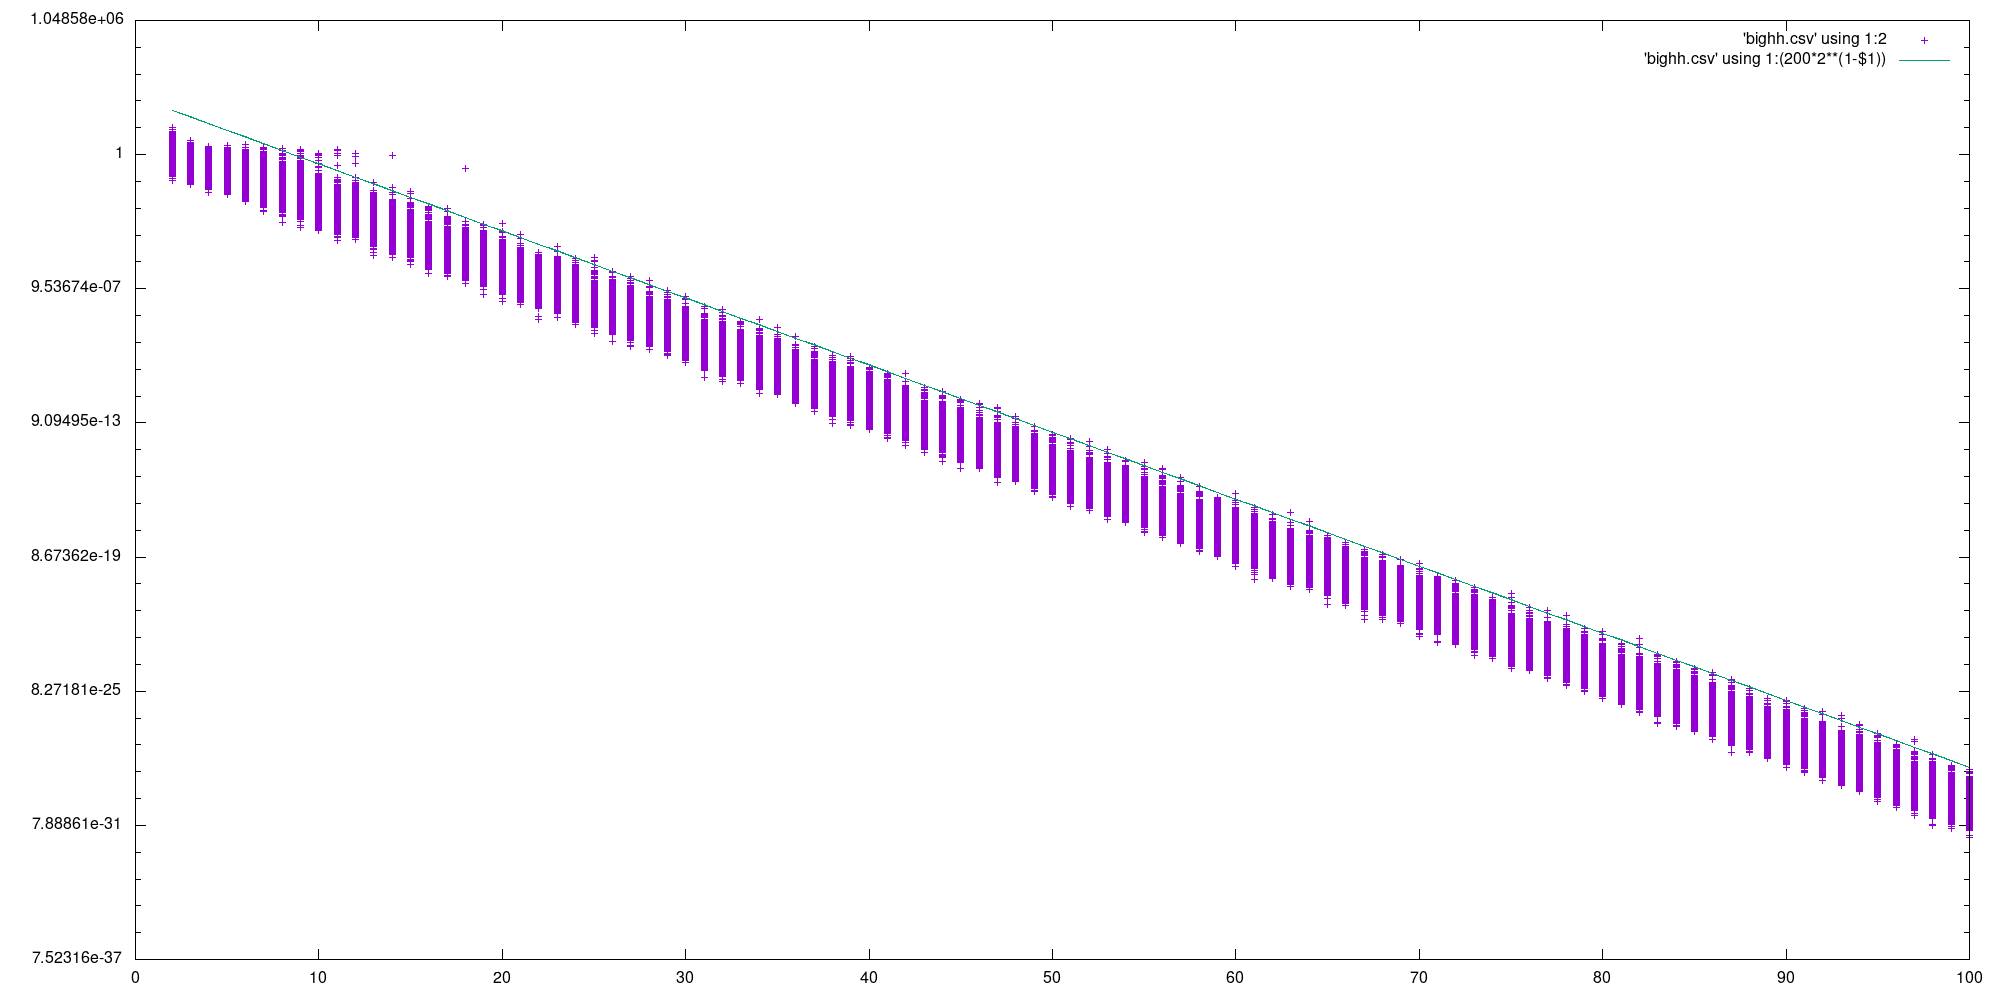
\includegraphics[width=\textwidth]{bighh}
	\caption{Experiments with Householder on different mantisa lengths.}
	\label{fig:errhh}
\end{figure}

The experiments shows that the error is decreased as the precision grows. The 
data shows a linear relationship between the length of the mantissa and the 
logarithm of the error.





\end{document}
